\chapter{Wprowadzenie do dziedziny}\label{chap:intr}

“Starożytni świat widzieli inaczej, mniej płasko”\cite{gbobrektvgry}. Dobrze obrazującym ówczesne postrzeganie przestrzeni przykładem jest mapa Imperium Rzymskiego,
pokazana na \ref{fig:mapaIR}. Czytanie jej dosłownie mija się z celem. Nie są na niej zachowane ani proporcje, ani strony świata. Mimo tego, że
basen Morza Śródziemnego został ówcześnie dosyć dokładnie oddany, “nie wydaje się, aby Rzymianom współczesna kartograficzna wierność była potrzebna”\cite{gbobrektvgry}.
“Dowódcy opierali się na swojej wiedzy, wiedzy wynajętych przewodników oraz informacjach zwiadowców i tubylców”\cite{gbobrektvgry}.
\begin{figure}[htbp]
    \centering
    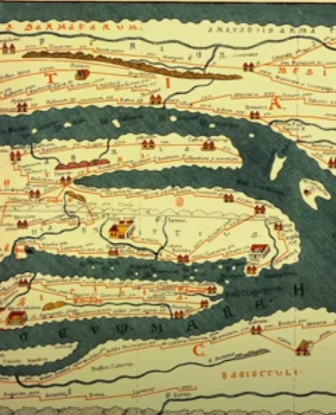
\includegraphics[width=0.5\textwidth]{images/mapaIR.png}
    \caption{Mapa basenu Morza Śródziemnego z czasów Imperium Rzymskiego}\label{fig:mapaIR}
\end{figure}
